\documentclass{scrreprt}

\usepackage{aligned-overset}
\usepackage{amsmath}
\usepackage{amssymb}
\usepackage{bm}
\usepackage[shortlabels]{enumitem}
\usepackage{hyperref}
\usepackage[utf8]{inputenc}
\usepackage{mathtools}
\usepackage{physics}
\usepackage{tabularx}
\usepackage{titling}
\usepackage{fancyhdr}
\usepackage{xfrac}
\usepackage{pgfplots}

\pgfplotsset{compat = newest}
\usepgfplotslibrary{fillbetween}

\author{Albina Oscherowa \\ Lukas Kamratzki \\ Karsten Lehmann}
\date{SoSe 2021}
\title{Hausaufgabe 06 \\Analysis - Weiterführende Konzepte}

\setlength{\headheight}{26pt}
\pagestyle{fancy}
\fancyhf{}
\lhead{\thetitle}
\rhead{\theauthor}
\lfoot{\thedate}
\rfoot{Seite \thepage}

\begin{document}

\section*{Hausaufgabe 1}

Untersuchen Sie, ob die Funktion
\[
  f \colon \mathbb{R}^2 \to \mathbb{R} \text{ mit }
  f\qty(x_1, x_2) \coloneqq \sin\qty(x_1) \cdot \ln\qty(2 + \sin(x_2))
\]
auf der Menge
\[
  K \coloneqq \qty{x = \qty(x_1, x_2) \in \mathbb{R}^2 \middle| \qty(0 \leq x_1) \land \qty(2\qty(x_2 - 2)^2 + x_1 \leq 4)}
\]
Maximum und Minimum besitzt. \\

\textit{Lsg.} Aus den Beschränkungen für $x_1$ und $x_2$ folgt
\[
  0 \leq x_1 \leq 4 \text{ und } 2 - \sqrt{2} \leq x_2 \leq 2 + \sqrt{2}
\]
$\Rightarrow K \subseteq [0, 4] \times [0, 4] \Rightarrow K$ ist beschränkt.

\begin{center}
  \begin{tikzpicture}[
      declare function={
        f(\x) = 2 * (2 - (\x - 2)^2);
      }
    ]
    \begin{axis}[
      axis lines=middle,
      xlabel=$x_2$,
      xmax = 3.7,
      xmin = 0.3,
      ylabel=$x_1$,
      ymax = 4.2,
      ymin = -0.2,
      ]
      \path[name path=axisa] (axis cs:0.586,0) -- (axis cs:3.414,0);
      \addplot[
        domain = 0.586:3.414,
        very thick,
        name path = f1,
        samples = 100,
        blue,
      ] {f(x)};
      \addplot[
        fill = blue!10,
        fill opacity = .5,
      ] fill between[of = f1 and axisa];
      \node at (2,1) {$K$};
    \end{axis}
  \end{tikzpicture}
\end{center}

Die Funktionen $g_1, g_2, g_3 \colon \mathbb{R}^2 \to \mathbb{R}$ mit
$g_1\qty(x_1, x_2) = x_1$, $g_2\qty(x_1, x_2) = x_2$ und
$g_2\qty(x_1, x_2) = 2\qty(x_2 - 2)^2 + x_1$ sind stetig.
Folglich sind die Mengen
\begin{flalign*}
  A_1 &\coloneqq g_1^{-1}([0, \infty)) = [0, \infty) \times \mathbb{R} & \\
  A_2 &\coloneqq g_2^{-1}([0, \infty)) = \mathbb{R} \times [0, \infty) & \\
  A_3 &\coloneqq g_3^{-1}((-\infty, 4]) =
  \qty{\qty(x_1, x_2) \in \mathbb{R}^2 \middle| \qty(x_1 \in \mathbb{R}) \land \qty(x_1 \leq 2\qty(2 - \qty(x_2 - 2)^2))}
\end{flalign*}
als Urbilder stetiger Funktionen abgeschlossener Mengen ebenfalls abgeschlossen.
Damit ist $K = A_1 \cap A_2 \cap A_3$ als Durchschnitt abgeschlossener Mengen
abgeschlossen $\Rightarrow K$ ist kompakt.

$f$ ist eine Komposition stetiger Funktionen
$\Rightarrow f$ ist stetig
$\Rightarrow f(K)$ ist kompakt.

Damit existieren $a, b \in K$ mit $f(a) \leq f(x) \leq f(b)$ für alle
$x \in K$.

\newpage
\section*{Hausaufgabe 2}

Seien $(M, d)$ ein metrischer Raum und $a \in M$ ein isolierter Punkt.

\noindent
Der Punkt $a \in M$ heißt isoliert, wenn ein $r > 0$ existiert, so dass
$B_d(a, r) \cap M = \qty{a}$.

\begin{enumerate}[a)]
\item Zeigen Sie, dass jede Funktion $f \colon M \to \mathbb{R}$ in $a$
  stetig ist. \\

  \textit{Lsg.} Eine Funktion $f \colon M \to \mathbb{R}$ heißt stetig in
  $a \in M$, wenn
  \[
    \forall \epsilon > 0 \exists \delta > 0 \forall b \in M
    \colon d(a, b) < \delta \Rightarrow \abs{f(a) - f(b)} < \epsilon
  \]
  Sei nun $\delta = \frac{r}{2}$, dann ist die Ungleichung
  $d(a, b) < \delta$ für $b \ne a$ falsch.
  Weiterhin ist $\abs{f(a) - f(a)} = 0$.
  Somit ist $f$ stetig in $a$ stetig.

\item Die Menge $M \coloneqq \qty{\frac{1}{n} \middle| n \in \mathbb{N}}$
  sei mit der von $(\mathbb{R}, \abs{\cdot})$ induzierten Metrik versehen.
  Geben Sie die Menge der stetigen Funktionen $f \colon M \to \mathbb{R}$
  an. \\

  \textit{Lsg.}
  $\frac{1}{n - 1} > \frac{1}{n} > \frac{1}{n + 1}, n \in \mathbb{N}$ und
  $\frac{1}{n} - \frac{1}{n \pm 1} > \frac{1}{2n(n + 1)}$.
  Somit ist jeder Punkt $a \in M$ isoliert mit
  $r = \frac{1}{\sfrac{2}{a}\qty(\sfrac{1}{a} + 1)}$.
  $\Rightarrow$ jede Funktion $f \colon M_0 \to \mathbb{R}$ ist in allen
  Punkten stetig.

\item $M_0 \coloneqq \qty{0} \cup M$ sei ebenfalls mit der von
  $(\mathbb{R}, \abs{\cdot})$ induzierten Metrik versehen.
  Geben Sie die Menge der stetigen Funktionen $f \colon M \to \mathbb{R}$
  an. \\

  \textit{Lsg.} $M_0 = \qty{0} \cup \qty{\frac{1}{n} \middle| n \in \mathbb{N}}$.
  Der Punkt $0$ ist nun nicht isoliert, da für jedes $r > 0$ ein
  $n \in \mathbb{N}$ mit $0 < \frac{1}{n} < r$ existiert.

  Somit sind Funktionen $f \colon M_0 \to \mathbb{R}$ stetig, die im Punkt $0$
  stetig sind, also:
  \[
    \forall \epsilon > 0 \exists \delta > 0 \forall x \in M_0
    \colon \abs{x} < \delta \Rightarrow \abs{f(0) - f(x)} < \epsilon
  \]

\end{enumerate}

\newpage
\section*{Hausaufgabe 3}

Es sei $M$ der Vektorraum aller reellen $2 \times 2$-Matrizen, d.h.
\[
  M \coloneqq \qty{A = \qty(\begin{array}{cc} a_{11} & a_{12} \\ a_{21} & a_{22}\end{array}) \middle| a_{ik} \in \mathbb{R}}
\]
Welche der folgenden Abbildungen $p_x \colon M \to \mathbb{R}$ sind Normen auf $M$?
\begin{enumerate}[a)]
\item $p_1(A) \coloneqq \det A$ \\

  \textit{Lsg.} Sei $A = \qty(\begin{array}{cc}0&1\\1&0\end{array}) \in M$,
  dann ist $p_2(A) = -1$, ein Widerspruch zu
  $\forall x \in M \colon \norm{x} \geq 0$.

  $\Rightarrow p_2$ ist keine Norm auf $M$.

\item $p_2(A) \coloneqq \abs{\det A}$ \\

  \textit{Lsg.} Sei $A = \qty(\begin{array}{cc}1&1\\1&1\end{array}) \in M$,
  dann ist $p_1(A) = 0$, ein Widerspruch zu
  $\forall x \in M \colon \norm{x} = 0 \iff x = 0$.

  $\Rightarrow p_1$ ist keine Norm auf $M$.

\item $p_3(A) \coloneqq \abs{a_{11}} + \abs{a_{12}} + \abs{a_{21}} + \abs{a_{22}}$ \\

  \textit{Lsg.}
  \begin{enumerate}[(i)]
  \item $\forall A \in M \colon p_3(A) \geq 0 \land p_3(A) = 0 \iff A = 0$ folgt aus der Definition des Betrags
  \item $\forall \lambda \in \mathbb{R}, A \in M \colon p_3(\lambda \cdot A) = \abs{\lambda} \cdot p_3(A)$ \\
    $\abs{\lambda a_{11}} + \abs{\lambda a_{12}} + \abs{\lambda a_{21}} + \abs{\lambda a_{22}} =
    \abs{\lambda} \cdot \qty(\abs{a_{11}} + \abs{a_{12}} + \abs{a_{21}} + \abs{a_{22}})$
  \item $\forall A, B \in M \colon p_3(A + B) \leq p_3(A) + p_3(B)$
    folgt aus der Dreiecksungleichung und Proposition 1.2.3 (d) der Vorlesung.
  \end{enumerate}
  $\Rightarrow p_3$ ist eine Norm auf $M$.

\item $p_4(A) \coloneqq \max\qty{\abs{a_{11}}, \abs{a_{12}}, \abs{a_{21}}, \abs{a_{22}}}$

  \textit{Lsg.}
  \begin{enumerate}[(i)]
  \item $\forall A \in M \colon p_3(A) \geq 0 \land p_3(A) = 0 \iff A = 0$ folgt aus der Definition des Betrags
  \item $\forall \lambda \in \mathbb{R}, A \in M \colon p_3(\lambda \cdot A) = \abs{\lambda} \cdot p_3(A)$
    folgt aus Proposition  1.2.3 (e) der Vorlesung.
  \item $\forall A, B \in M \colon p_3(A + B) \leq p_3(A) + p_3(B)$
    Seine $a \in A, b \in B$ beliebig, dann folgt aus
    $\abs{a} \leq p_4(A)$ und $\abs{b} \leq p_4(B)$, dass
    $\abs{a} + \abs{b} \leq p_4(A) + p_4(B) \Rightarrow p_4(A + B) \leq p_4(A) + p_4(B)$
  \end{enumerate}
  $\Rightarrow p_4$ ist eine Norm auf $M$.
\end{enumerate}

\end{document}